\section{Case Study: the generic mesa model}

We will study a class of reaction-diffusion equations, that under some conditions exhibit mesa-type solutions. We will construct a general multi-mesa solution, and study its stability.

The system we will study is the following system of reaction diffusion equations:
% 
\begin{equation}
\label{eqn:gms1}
\begin{split}
\begin{aligned}
	u_t &= \Ep^2\De u + f(u,v) \\
	\tau v_t &= \frac{\DD}{\Ep}\De v + g(u,v),
\end{aligned}
\end{split}
\end{equation}
% 
with homogeneous Neumann boundary conditions on $x\in[0,1]\times[0,d_0]$. We consider the limit where $\Ep\ll 1$, and regard all the other constants as being $O(1)$. 

\subsection{Construction of the solution in the near-shadow limit}

(Reference to McKay and Kolokolnikov)

We want to construct a $K-$stripe stationary mesa solution on $x\in[0,1]$. A mesa structure is characterized as a function $u(x)\sim u_+$ on $-l<x<l$, and $u(x)\sim u_-$ on $l<|x|<L$; with $u_+>u_-$, and both values joined by a sharp interface.

The mesa pattern will be formed by two back-to-back interfaces. We will start by constructing a solution on $[0,L]$, with the interface centred at $x=l$. A full mesa solution can then be constructed by adding an even reflection (see figure \ref{fig:single_mesa}), and a $K-$mesa solution will simply be $K$ copies, or $2K$ interfaces. 
% 
% \begin{figure}[htb]
% \begin{center}
% 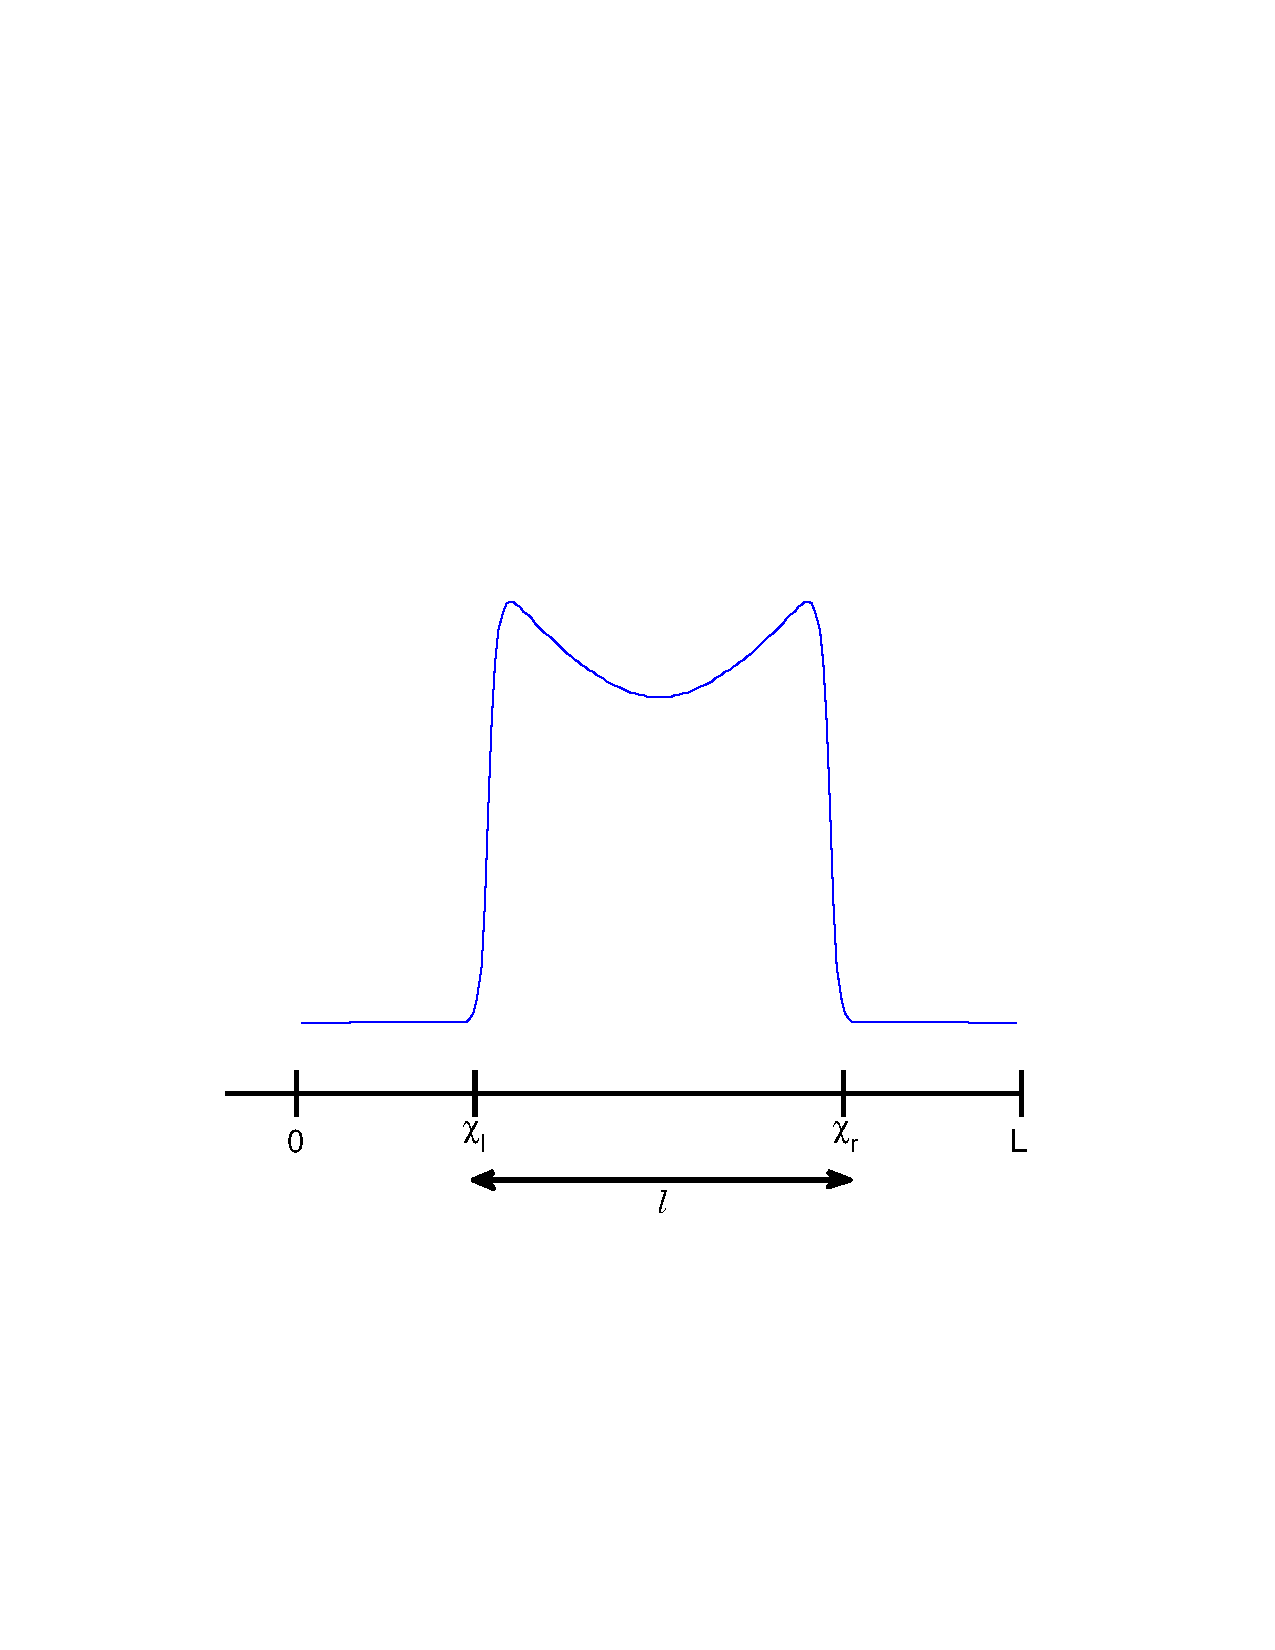
\includegraphics[width=4in]{single_mesa}
% \caption{A typical mesa profile in the stationary solution $v(x)$. The left and right edges of the mesa are labelled as $\chi_l$ and $\chi_r$ respectively; and the length of the mesa section is $l$ (***add multi-mesa picture)) *** wrong fig.}
% \label{fig:single_mesa}
% \end{center}
% \end{figure}
% 
The stationary equation we want to solve is
% 
\begin{equation}
\label{eqn:gms_stat}
\begin{split}
\begin{aligned}
	0 &= \Ep^2 u_{xx}+ f(u,v),\qquad &u_x(-L)=u_x(L)=0, \\
	0 &= \frac{\DD}{\Ep}v_{xx}+ g(u,v),\qquad &v_x(-L)=v_x(L)=0.
\end{aligned}
\end{split}
\end{equation}
% 
To first order, we have $v_{xx}=0$. Applying the Neumann boundary condition, we have then that $v\sim\VV$, and the value of the constant can be estimated by integrating over the whole domain. The resulting equation is	
% 
\begin{equation}
\label{eqn:v_first_order}
  0 = \int_0^Lg(u,\VV)dx,
\end{equation}
% 
with $v=\VV$ constant.

Now, we are looking for a heteroclinic connection in $u$ as the transition mechanism connecting $u=u_+$ to $u=u_-$. This imposes the algebraic constraint that $f(u_+,V)\equiv f_+ = 0$, and $ f(u_-,V) \equiv f_- = 0$, which has to be satisfied together with the Maxwell line condition \cite{maxwell1994} $\int_{u_-}^{u_+} f(w,\VV)dw = 0$. For both branches to be stable we also require $f_u(u_{\pm},\VV)<0$. Solving the algebraic system determines $u_{\pm}$, and $v_0=\VV$.

In the inner region near the interface of the mesa, we have that $v\sim\VV$, and we do a change of variables for $y=\Ep^{-1}(x-l)$, and $u(x)\sim U_0(\frac{x-l}{\Ep})$ . Integrating \eqref{eqn:v_first_order} in two parts across the interface yields the following result
% 
\begin{equation*}
\label{eqn:w_eqn}
\begin{split}
\begin{aligned}
  0 &= \frac{D}{\Ep}\int_0^lv_{xx}+\int_0^lg(u,\VV)dx\quad&\Rightarrow&\qquad \frac{D}{\Ep}v_x(l^-)=-lg_+,\\
  0 &= \frac{D}{\Ep}\int_l^Lv_{xx}+\int_l^Lg(u,\VV)dx\quad&\Rightarrow&\qquad \frac{D}{\Ep}v_x(l^+)=(L-l)g_-.
\end{aligned}
\end{split}
\end{equation*}

Since the $v$ solution doesn't have sharp interfaces, we have then that to first order
% 
\begin{equation}
\label{eqn:l_eqn}
\begin{split}
  l = \frac{g_-}{g_- - g_+}L + O(\Ep).
\begin{aligned}
\end{aligned}
\end{split}
\end{equation}
% 

Furthermore, since $0<l<L$, we have the consistency condition
% 
\begin{equation*}
  0<\frac{g_-}{g_- - g_+}<1,
\end{equation*}
% 
and as with $f_{\pm}$, we have that $g_{\pm} \equiv g(u_{\pm},\VV)$.

We will divide the half-mesa branch into three regions: the outer part on the mesa plateau, $0<x<l$; the outer part of the mesa beyond the plateau, $x>l$; and the internal layer around $x=l$ bridging the two outer regions.

To zoom into the inner layer we let $y=\frac{x-l}{\Ep},\hspace{1ex} u(\Ep y+l)\equiv U(y),\hspace{1ex} v(\Ep y+l)\equiv V(y)$; which when substituted into \eqref{eqn:gms_stat} results in
% 
\begin{equation}
\label{eqn:gms_layer}
\begin{split}
\begin{aligned}
	&U_{yy}+ f(U,V) =0,\qquad &\infty<y<\infty,\qquad &U\rightarrow U_{\pm} \text{ as } y\rightarrow\mp\infty,\\
	&V_{yy}+ \frac{\Ep^3}{\DD} g(U,V)=0,\qquad &\infty<y<\infty,\qquad &V\rightarrow V_{\pm} \text{ as } y\rightarrow\mp\infty.
\end{aligned}
\end{split}
\end{equation}
% 

In the outer region, $0<x<l$, we have
% 
\begin{equation*}
% \label{eqn:gms_outer1}
\begin{split}
\begin{aligned}
	&f(u,v) = 0,\qquad &u_x(0)=0,\\
	&v_{xx}+ \frac{\Ep}{\DD} g(u,v) = 0,\qquad &v_x(0)=0.
\end{aligned}
\end{split}
\end{equation*}
% 
with the boundary conditions stemming from the even symmetry imposed on the mesas. Similarly, for the region $x>l$ we have
% 
\begin{equation}
\label{eqn:gms_outer2}
\begin{split}
\begin{aligned}
	&f(u,v) = 0,\qquad &u_x(L)=0,\\
	&v_{xx} + \frac{\Ep}{\DD} g(u,v) = 0,\qquad &v_x(L)=0.
\end{aligned}
\end{split}
\end{equation}
% 

Performing an asymptotic expansion $u = u_- + \frac{\Ep}{\DD}u_1 + \cdots, \hspace{1ex} v = \VV + \frac{\Ep}{\DD}v_1 + \cdots$, and substituting into a Taylor expansion of $f(u,v)$ in \eqref{eqn:gms_outer2}, we obtain
% 
\begin{equation*}
% \label{eqn:taylor_f}
\begin{split}
\begin{aligned}
	&f(u_-,\VV) + \frac{\Ep}{\DD}(f_u^-u_1 + f_v^-v_1) + \cdots = 0,\\
\end{aligned}
\end{split}
\end{equation*}
%
thus $u_1 = -\frac{f_v^-}{f_u^-}v_1$, where $f_v^{\pm} = f_v(u_{\pm},\VV)$, and  $f_u^{\pm} = f_u(u_{\pm},\VV)$.

From \eqref{eqn:gms_outer2} we also obtain that
% 
\begin{equation}
\label{eqn:v_outer}
\begin{split}
\begin{aligned}
	&v_{1xx} = -g_-,\qquad\text{on }l<x<L,\qquad\text{with }g_- = g(u_-,\VV),\\
	&v_{1x}(L) = 0,\qquad v_1(l^+)=v_{1-},
\end{aligned}
\end{split}
\end{equation}
%
where we have imposed the boundary condition $v_1(l^+) = v_{1-}$ in terms of an unknown constant $v_{1-}$ to be calculated later.

The solution in this region is
% 
\begin{equation}
\label{eqn:v1}
\begin{split}
\begin{aligned}
	v_1(x) = -g_-\left(\frac{1}{2}(x-L)^2-\frac{1}{2}(L-l)^2\right) + v_{1-},
\end{aligned}
\end{split}
\end{equation}
%
therefore we have that in the outer region $l<x<L$ 
% 
\begin{equation}
\label{eqn:uv_outer2}
\begin{split}
\begin{aligned}
	&u\sim u_- + \frac{\Ep}{\DD}\left(-\frac{f_v^-}{g_u^-}v_1(x) \right),\\
	&v\sim \VV + \frac{\Ep}{\DD}v_1(x).
\end{aligned}
\end{split}
\end{equation}
%
Either by derivating \eqref{eqn:uv_outer2}, or integrating \eqref{eqn:v_outer} over $l<x<L$ we get that $v_{1x}(l^+)\equiv v_{1-}' = g_-(L-l)$.

An analogous calculation on the outer region $0<x<l$ yields 
% 
\begin{equation*}
% \label{eqn:uv_outer1}
\begin{split}
\begin{aligned}
	&u\sim u_+ + \frac{\Ep}{\DD}\left(-\frac{f_v^+}{g_u^+}v_1(x) \right),\\
	&v\sim \VV + \frac{\Ep}{\DD}v_1(x),\quad\text{with}\quad v_1(x) = -g_+\left(\frac{1}{2}x^2-\frac{l^2}{2} \right) + v_{1+},
\end{aligned}
\end{split}
\end{equation*}
%
again with a boundary condition $v_1(l^-)=v_{1+}$ in terms of an unknown constant to be found. 

% 
\begin{equation}
\label{eqn:matching_inner}
\begin{split}
\begin{aligned}
	v_{1x}(l^-)\equiv v_{1+}' &= -g_+l,\\
	v_{1x}(l^+)\equiv v_{1-}' &= g_-(L-l).
\end{aligned}
\end{split}
\end{equation}
%

Taylor expanding both solutions near $x=l^{\pm}$ provides matching conditions for the inner solution. The problem for the inner layer, in terms of the variable $y=\Ep^{-1}(x-l)$, is
% 
\begin{equation*}
% \label{eqn:uv_inner2}
\begin{split}
\begin{aligned}
	&U_{yy}+f(U,V)=0,\quad -\infty<y<\infty,\quad U\sim u_{\pm}-\frac{\Ep}{\DD}\frac{f_v^{\pm}}{f_u^{\pm}}v_{1\pm}\text{ as }y\rightarrow\mp\infty ,\\
	&V_{yy}=-\frac{\Ep^3}{\DD}g(U,V),\quad -\infty<y<\infty,\quad V\sim \VV+\frac{\Ep}{\DD}(V_{1\pm}+\Ep yV_{1\pm}') \text{ as }y\rightarrow\mp\infty.
\end{aligned}
\end{split}
\end{equation*}
%

Expanding the inner solution, $U = U_0 + \frac{\Ep}{\DD}U_1 + \cdots,\hspace{1ex} V = V_0 + \frac{\Ep}{\DD}V_1 + \cdots$, we get
% 
\begin{equation*}
% \label{eqn:uv_inner1}
\begin{split}
\begin{aligned}
	\LL(U_1) &= U_{1yy}+f_U(U_0,V_0)U_1=-f_V(U_0,V_0)V_1,\\
	V_{1yy} &= 0.
\end{aligned}
\end{split}
\end{equation*}
%

The matching condition for $V_1 = h_1y+h_2$ is $V_1\sim v_{1\pm}\text{ as }y\rightarrow\mp\infty$. Thus we must have that $h_1=0$, and $h_2 = v_{1+} = v_{1-} = V_1$.

We can obtain a solvability condition since by translational invariance we have that $\LL(U_0') = 0$. Hence
% 
\begin{equation*}
% \label{eqn:solva1}
\begin{split}
\begin{aligned}
	\int_{-\infty}^{\infty}(U_0'\LL U_1 - U_1\LL U_0')dy = -V_1\int_{-\infty}^{\infty}U_0'f_V(U_0,V_0)dy = 0.
\end{aligned}
\end{split}
\end{equation*}
%

We can conclude then that if $f_V\neq0$ then $V_1=0$, thus $V_{1\pm}=0$. We also have then that $U_1 = cU_0'$, and without loss of generality we take $c=0$.

To $O(\Ep)$ we have then
% 
\begin{equation}
\label{eqn:u_outer}
	\begin{split}
	v(x) &= \left\{
	\begin{matrix}
	  \VV + \frac{\Ep}{2\DD}\left(g_-(x-L)^2 + g_-(L-l)^2 \right),&l<x<L,\\
	  \VV - \frac{\Ep}{2\DD}g_+(x^2-l^2),\hspace{1in}&0<x<l.
	\end{matrix}\right.\\
	u(x) &= \left\{
	\begin{matrix}
	  u_- + O(\frac{\Ep^2}{\DD}),\hspace{1.43in}&l<x<L,\\
	  u_+ + O(\frac{\Ep^2}{\DD}),\hspace{1.42in} &0<x<l.
	\end{matrix}\right.\\
	\end{split}
\end{equation}
% 

In the inner region we expand to second order, $u=U_0 + \frac{\Ep^2}{\DD}U_2+\cdots,\hspace{1ex}, v = \VV + \frac{\Ep^2}{\DD}V_2+\cdots$, and get
% 
\begin{equation*}
% \label{eqn:uv_inner_O2}
\begin{split}
\begin{aligned}
	\LL(U_2) &= U_{2yy}+f_U(U_0,V_0)U_2=-f_V(U_0,V_0)V_2,\\
	V_{2yy} &= 0,
\end{aligned}
\end{split}
\end{equation*}
%
with the matching condition that $V_2\sim yv_{1\pm}'\text{ as }y\rightarrow\mp\infty$, and $v_1$ the $O(\Ep/\DD)$ term for $v(x)$ in \eqref{eqn:u_outer}.

We must have then that $V_2(y) = H_{20} + yH_{21}$, and we can conclude that $H_{21} = V_{1+}' = V_{1-}'$. Using \eqref{eqn:matching_inner}, we can now recover the result from \eqref{eqn:l_eqn}:
% 
\begin{equation*}
	g_-(L-l) = -g_+l\qquad \rightarrow \qquad l=\frac{g_-}{g_- - g_+}L.
\end{equation*}
% 

The constant $H_{20}$ can be found in terms of $H_{21}$ via a solvability condition, since $\LL U_0' = 0$, and 
% 
\begin{equation*}
	\LL U_2 = U_{2yy} + f_U(U_0,V_0)U_2 = -f_V(U_0,V_0)(H_{20}+yH_{21}),\\
\end{equation*}
% 

We have then that
% 
\begin{equation*}
\begin{split}
\begin{aligned}
  \int_{-\infty}^{\infty}(H_{20}+yH_{21})U_0'f_V(U_0,V_0)dy = 0,\\
	\text{hence}\quad H_{20} = -V_{1\pm}'\frac{\int_{-\infty}^{\infty}yU_0'f_V(U_0,V_0)dy}{\int_{-\infty}^{\infty}U_0'f_V(U_0,V_0)dy}
\end{aligned}
\end{split}
\end{equation*}
% 

In the outer expansion, $v(x) = \VV + \frac{\Ep}{\DD}v_1 + \frac{\Ep^2}{\DD}v_2$, we require then that $v_2(l) = H_{20}$.
